\documentclass[12pt]{article}
\usepackage{amsmath}
\usepackage{physics}
\usepackage[backend=biber, style=chem-acs]{biblatex}
\usepackage{graphicx}
\author{Patryk Kozlowski}
\title{Fall Quarter Report}
\date{\today}
\addbibresource{refs.bib}
\begin{document}
\maketitle
\section{Notation}
In the MO basis, $p,q,r,s,...$ are used for general orbitals. $i,j,k,l,...$ are used for occupied orbitals. $a,b,c,d,...$ are used for virtual orbitals.
\section{Theory}
There are two main equations that I have been working with this quarter. They are described below.
\subsection{Self Energy}
\begin{equation}
    \Sigma_{pp}^{\text{corr}}(\omega) = \sum_{\mu }^{\text{RPA}}\left(\sum_{i}^{\text{occupied}} \frac{V_{pi}^{\mu }V_{ip}^{\mu }}{\omega -(\varepsilon _{i}-\Omega  _{\mu })}+ \sum_{a}^{\text{virtual}} \frac{V_{pa}^{\mu }V_{ap}^{\mu }}{\omega -(\varepsilon _{a}+\Omega  _{\mu })}\right)
\end{equation}
I have implemented the diagonal of the real part of the correlation self-energy. The $V$ and $\Omega$ are the excitation vectors and energies, respectively, from a previous TD-DFT routine; the direct Tamm-Dancoff approximation (dTDA) and the direct Random Phase Approximation (dRPA) were used here. $\omega$ is my input frequency and the $\varepsilon$ are the orbital energies from my previous mean-field calculation.
\subsection{Iterative $G_0W_{0}$ Procedure}
\begin{equation}
    \delta_{pq}F_{pq}^{HF}[\gamma^{MF}] + \Sigma_{pp}^{corr}(\varepsilon_{p}^{QP}) = \varepsilon_{p}^{QP}
\end{equation}
I have also implemented the iterative procedure to obtain my quasiparticle energies. The first term indicates that I am using the corresponding diagonal element at the orbital index of the HF Fock matrix evaluated at the mean-field density. In the second term, I am inputting quasiparticle energies into the self-energy from equation 1. The output of this equation is a new quasiparticle energy that I use in the next iteration. This process is iterated until convergence. In my very first iteration, the $\varepsilon_{p}^{QP}$ that I input into my $\Sigma_{pp}^{corr}$ is just the orbital energy from my mean-field calculation.
\newpage
\section{Results}
I have been working with the HOMO of the water molecule with HF or DFT@PBE as my mean field object. I have plotted my self-energy computed for a wide range of frequencies. The line at $\omega - \varepsilon^{HF}$ should intersect with my self-energy at the same quasiparticle energy that I get from my iterative procedure, and indeed this is the case.
\begin{figure}[h]
    \centering
    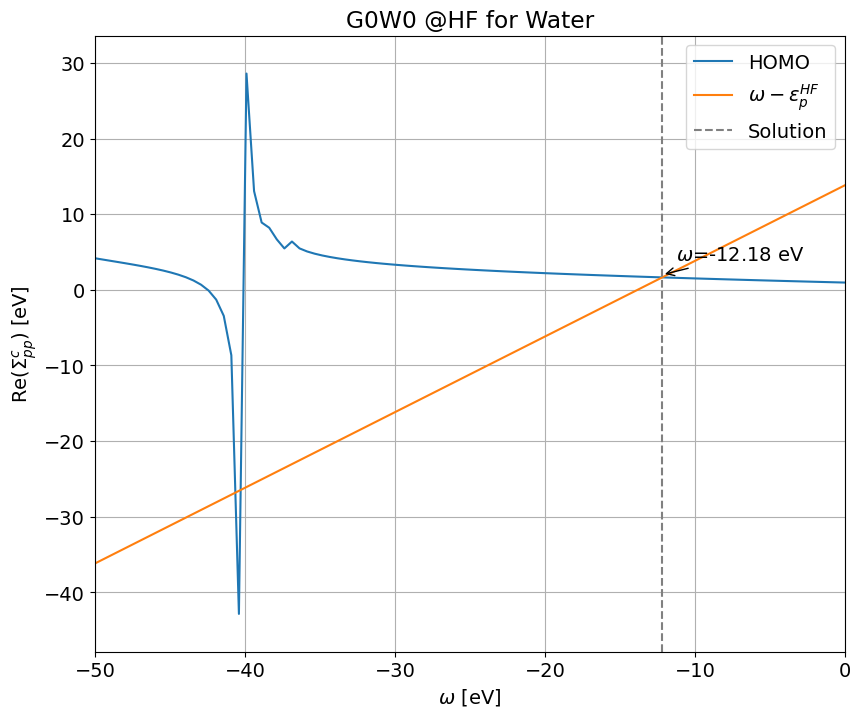
\includegraphics[width=\textwidth]{correlation_energies.png}
\end{figure}
Also, at around $\omega$ = -40 eV, one can observe a pole structure. This is a derivate discontinuity in my self-energy that would pose problems for my iterative procedure if the quasiparticle energy of the orbital that I was looking for was close to this value.
\end{document}